\documentclass[]{tufte-handout}

% ams
\usepackage{amssymb,amsmath}

\usepackage{ifxetex,ifluatex}
\usepackage{fixltx2e} % provides \textsubscript
\ifnum 0\ifxetex 1\fi\ifluatex 1\fi=0 % if pdftex
  \usepackage[T1]{fontenc}
  \usepackage[utf8]{inputenc}
\else % if luatex or xelatex
  \makeatletter
  \@ifpackageloaded{fontspec}{}{\usepackage{fontspec}}
  \makeatother
  \defaultfontfeatures{Ligatures=TeX,Scale=MatchLowercase}
  \makeatletter
  \@ifpackageloaded{soul}{
     \renewcommand\allcapsspacing[1]{{\addfontfeature{LetterSpace=15}#1}}
     \renewcommand\smallcapsspacing[1]{{\addfontfeature{LetterSpace=10}#1}}
   }{}
  \makeatother

\fi

% graphix
\usepackage{graphicx}
\setkeys{Gin}{width=\linewidth,totalheight=\textheight,keepaspectratio}

% booktabs
\usepackage{booktabs}

% url
\usepackage{url}

% hyperref
\usepackage{hyperref}

% units.
\usepackage{units}


\setcounter{secnumdepth}{-1}

% citations


% pandoc syntax highlighting
\usepackage{color}
\usepackage{fancyvrb}
\newcommand{\VerbBar}{|}
\newcommand{\VERB}{\Verb[commandchars=\\\{\}]}
\DefineVerbatimEnvironment{Highlighting}{Verbatim}{commandchars=\\\{\}}
% Add ',fontsize=\small' for more characters per line
\newenvironment{Shaded}{}{}
\newcommand{\AlertTok}[1]{\textcolor[rgb]{1.00,0.00,0.00}{\textbf{#1}}}
\newcommand{\AnnotationTok}[1]{\textcolor[rgb]{0.38,0.63,0.69}{\textbf{\textit{#1}}}}
\newcommand{\AttributeTok}[1]{\textcolor[rgb]{0.49,0.56,0.16}{#1}}
\newcommand{\BaseNTok}[1]{\textcolor[rgb]{0.25,0.63,0.44}{#1}}
\newcommand{\BuiltInTok}[1]{\textcolor[rgb]{0.00,0.50,0.00}{#1}}
\newcommand{\CharTok}[1]{\textcolor[rgb]{0.25,0.44,0.63}{#1}}
\newcommand{\CommentTok}[1]{\textcolor[rgb]{0.38,0.63,0.69}{\textit{#1}}}
\newcommand{\CommentVarTok}[1]{\textcolor[rgb]{0.38,0.63,0.69}{\textbf{\textit{#1}}}}
\newcommand{\ConstantTok}[1]{\textcolor[rgb]{0.53,0.00,0.00}{#1}}
\newcommand{\ControlFlowTok}[1]{\textcolor[rgb]{0.00,0.44,0.13}{\textbf{#1}}}
\newcommand{\DataTypeTok}[1]{\textcolor[rgb]{0.56,0.13,0.00}{#1}}
\newcommand{\DecValTok}[1]{\textcolor[rgb]{0.25,0.63,0.44}{#1}}
\newcommand{\DocumentationTok}[1]{\textcolor[rgb]{0.73,0.13,0.13}{\textit{#1}}}
\newcommand{\ErrorTok}[1]{\textcolor[rgb]{1.00,0.00,0.00}{\textbf{#1}}}
\newcommand{\ExtensionTok}[1]{#1}
\newcommand{\FloatTok}[1]{\textcolor[rgb]{0.25,0.63,0.44}{#1}}
\newcommand{\FunctionTok}[1]{\textcolor[rgb]{0.02,0.16,0.49}{#1}}
\newcommand{\ImportTok}[1]{\textcolor[rgb]{0.00,0.50,0.00}{\textbf{#1}}}
\newcommand{\InformationTok}[1]{\textcolor[rgb]{0.38,0.63,0.69}{\textbf{\textit{#1}}}}
\newcommand{\KeywordTok}[1]{\textcolor[rgb]{0.00,0.44,0.13}{\textbf{#1}}}
\newcommand{\NormalTok}[1]{#1}
\newcommand{\OperatorTok}[1]{\textcolor[rgb]{0.40,0.40,0.40}{#1}}
\newcommand{\OtherTok}[1]{\textcolor[rgb]{0.00,0.44,0.13}{#1}}
\newcommand{\PreprocessorTok}[1]{\textcolor[rgb]{0.74,0.48,0.00}{#1}}
\newcommand{\RegionMarkerTok}[1]{#1}
\newcommand{\SpecialCharTok}[1]{\textcolor[rgb]{0.25,0.44,0.63}{#1}}
\newcommand{\SpecialStringTok}[1]{\textcolor[rgb]{0.73,0.40,0.53}{#1}}
\newcommand{\StringTok}[1]{\textcolor[rgb]{0.25,0.44,0.63}{#1}}
\newcommand{\VariableTok}[1]{\textcolor[rgb]{0.10,0.09,0.49}{#1}}
\newcommand{\VerbatimStringTok}[1]{\textcolor[rgb]{0.25,0.44,0.63}{#1}}
\newcommand{\WarningTok}[1]{\textcolor[rgb]{0.38,0.63,0.69}{\textbf{\textit{#1}}}}

% table with pandoc

% multiplecol
\usepackage{multicol}

% strikeout
\usepackage[normalem]{ulem}

% morefloats
\usepackage{morefloats}


% tightlist macro required by pandoc >= 1.14
\providecommand{\tightlist}{%
  \setlength{\itemsep}{0pt}\setlength{\parskip}{0pt}}

% title / author / date
\title{Survival Basics: Censoring and Discrete Hazards}
\author{by Elie Gurarie}
\date{2024-09-16}


\begin{document}

\maketitle




Survival analysis models time-to-event as an outcome (e.g.~time to
death, how long do you wait for an animal to appear in a camera trap,
when will an earthquake strike, when will a mango fall, etc). There are,
in short, lots of ecological applications. But the biggest by far is, in
fact, modeling survival.

The goals in this lecture are to get an intuition for why time-to-event
data is fundamentally different than other kinds of observations, and -
on the basis of a simple experiment - get intuition for the \emph{hazard
function} and \emph{censored data} and how to estimate those using
maximum likelihood.

\section{Discrete Hazard process}\label{discrete-hazard-process}

We rolled dice - 52 to be precise - each until we got a 6. Each roll
represented a year. Once a \textbf{6} was rolled, the die was dead and
removed. Like with these
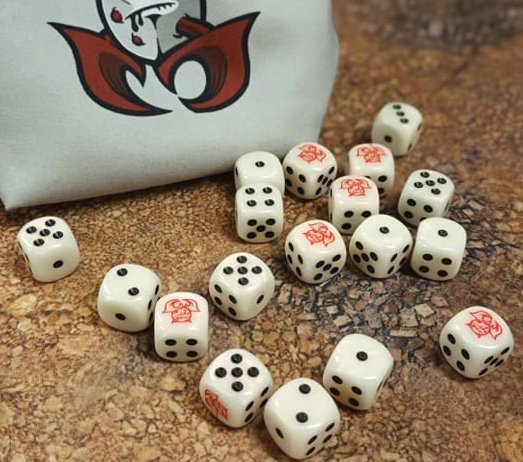
\includegraphics{lectures/Survival/lethaldice.jpg}

Here are the data:

\begin{Shaded}
\begin{Highlighting}[]
\FunctionTok{mean}\NormalTok{(X)}
\end{Highlighting}
\end{Shaded}

\begin{verbatim}
## [1] 7.211538
\end{verbatim}

\begin{Shaded}
\begin{Highlighting}[]
\FunctionTok{plot}\NormalTok{(}\FunctionTok{table}\NormalTok{(X), }\AttributeTok{type =} \StringTok{"h"}\NormalTok{)}
\end{Highlighting}
\end{Shaded}

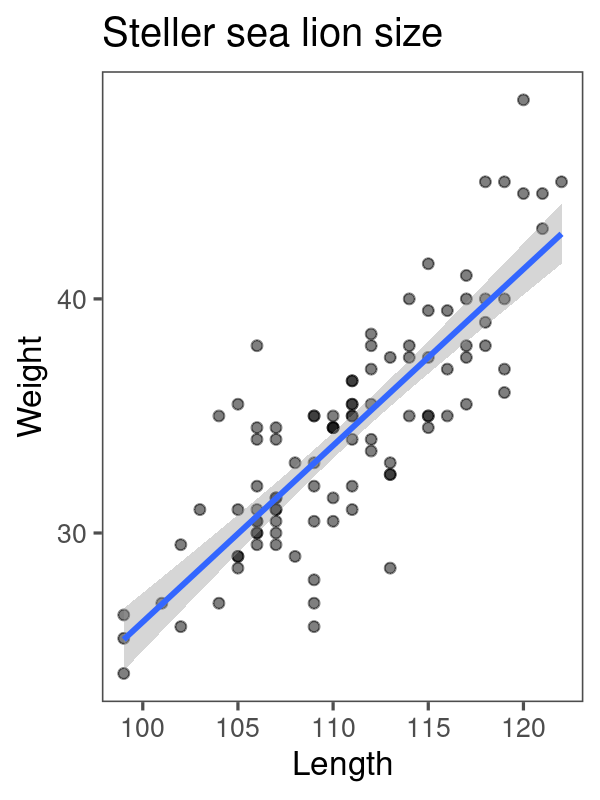
\includegraphics{Lecture1_files/figure-latex/unnamed-chunk-2-1}

If you like, you can also simulate this process:

\begin{Shaded}
\begin{Highlighting}[]
\NormalTok{X }\OtherTok{\textless{}{-}} \FunctionTok{rep}\NormalTok{(}\ConstantTok{NA}\NormalTok{, }\DecValTok{50}\NormalTok{)}
\ControlFlowTok{for}\NormalTok{(i }\ControlFlowTok{in} \DecValTok{1}\SpecialCharTok{:}\FunctionTok{length}\NormalTok{(X))\{}
\NormalTok{    rolls }\OtherTok{\textless{}{-}} \DecValTok{0}
\NormalTok{    x }\OtherTok{\textless{}{-}} \DecValTok{0}
    \ControlFlowTok{while}\NormalTok{(x }\SpecialCharTok{!=} \DecValTok{6}\NormalTok{)\{}
\NormalTok{        rolls }\OtherTok{\textless{}{-}}\NormalTok{ rolls}\SpecialCharTok{+}\DecValTok{1}
\NormalTok{        x }\OtherTok{\textless{}{-}} \FunctionTok{sample}\NormalTok{(}\DecValTok{1}\SpecialCharTok{:}\DecValTok{6}\NormalTok{,}\DecValTok{1}\NormalTok{)}
\NormalTok{    \}}
\NormalTok{    X[i] }\OtherTok{\textless{}{-}}\NormalTok{ rolls}
\NormalTok{\}}
\end{Highlighting}
\end{Shaded}

\subsection{Probability distribution}\label{probability-distribution}

The probability mass function of mortality time is:

\[Pr(X = x) = f(x|p) = p(1-p)^{x-1}\]

This can be reasoned out, but also has a name, the
\href{https://en.wikipedia.org/wiki/Negative_binomial_distribution}{negative
binomial distribution}: \(X \sim \text{NegBinom}(p)\)\footnote{\emph{Important
  note:} the standard definition of the negative binomial is
  \emph{number of failures before first success}, so it includes 0,
  whereas in our definition if the event dies in the first attempt,
  that's a 1, not a 0, so technically: \(X+1 \sim \text{NegBinom}(p)\).
  This becomes important later.}.

\subsection{Likelihood function}\label{likelihood-function}

\[{\cal L}(p|{\bf X}) = \prod_{i=1}^n f(X_i|p)\]

log-likelihood:

\[\begin{align} {\cal l}(p|{\bf X}) &= \sum (X_i-1) \log(1-p) + n\log(p) \\
& = n\log(p) + \left(\sum X_i - n\right) \log(1-p) \end{align}\]

\begin{Shaded}
\begin{Highlighting}[]
\NormalTok{p.ll }\OtherTok{\textless{}{-}} \ControlFlowTok{function}\NormalTok{(p, X)\{}
\NormalTok{  n }\OtherTok{\textless{}{-}} \FunctionTok{length}\NormalTok{(X)}
\NormalTok{  n}\SpecialCharTok{*}\FunctionTok{log}\NormalTok{(p) }\SpecialCharTok{+}\NormalTok{ (}\FunctionTok{sum}\NormalTok{(X)}\SpecialCharTok{{-}}\NormalTok{n) }\SpecialCharTok{*} \FunctionTok{log}\NormalTok{(}\DecValTok{1}\SpecialCharTok{{-}}\NormalTok{p)}
\NormalTok{\}}
\FunctionTok{curve}\NormalTok{(}\FunctionTok{p.ll}\NormalTok{(x, }\AttributeTok{X =}\NormalTok{ X), }\AttributeTok{xlab =} \StringTok{"p"}\NormalTok{)}
\end{Highlighting}
\end{Shaded}

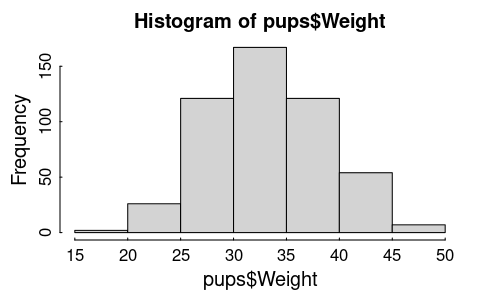
\includegraphics{Lecture1_files/figure-latex/unnamed-chunk-4-1}

\subsection{Maximum likelihood
estimate}\label{maximum-likelihood-estimate}

The maximum likelihood estimate is where this curve is - at a maximum!

\begin{Shaded}
\begin{Highlighting}[]
\NormalTok{(p.hat }\OtherTok{\textless{}{-}} \FunctionTok{optimize}\NormalTok{(p.ll, }\FunctionTok{c}\NormalTok{(}\DecValTok{0}\NormalTok{,}\DecValTok{1}\NormalTok{), }\AttributeTok{X =}\NormalTok{ X, }\AttributeTok{maximum =} \ConstantTok{TRUE}\NormalTok{))}
\end{Highlighting}
\end{Shaded}

\begin{verbatim}
## $maximum
## [1] 0.1386616
## 
## $objective
## [1] -150.9509
\end{verbatim}

Plot the maximum

\begin{Shaded}
\begin{Highlighting}[]
\FunctionTok{curve}\NormalTok{(}\FunctionTok{p.ll}\NormalTok{(x, }\AttributeTok{X =}\NormalTok{ X), }\AttributeTok{xlab =} \StringTok{"p"}\NormalTok{)}
\FunctionTok{abline}\NormalTok{(}\AttributeTok{v =}\NormalTok{ p.hat, }\AttributeTok{lwd =} \DecValTok{2}\NormalTok{, }\AttributeTok{col =} \DecValTok{2}\NormalTok{)}
\end{Highlighting}
\end{Shaded}

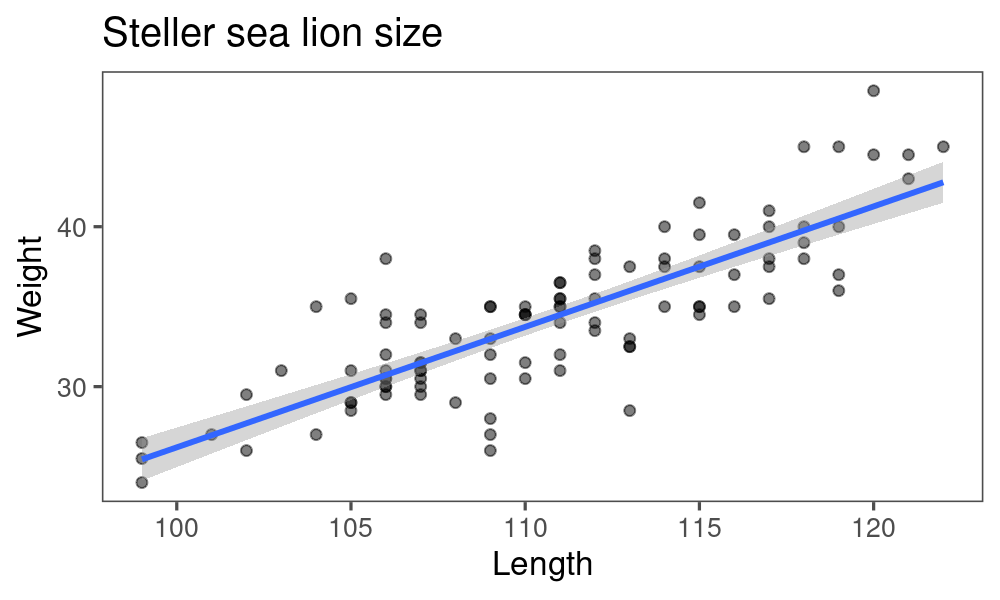
\includegraphics{Lecture1_files/figure-latex/unnamed-chunk-6-1}

But now we can also get a confidence interval, using the all important
\emph{Hessian}. Recall that for a maximum likelihood estimate
\(\widehat{\theta}\) , an asymptotic estimate of its variance is given
by \[\sigma^2_{\hat\theta} = {-1\over d^2l(\hat\theta)/d\theta^2}\]

i.e., the greater the (negative) curvature, the smaller the standard
error. Here's one way to compute this:

\begin{Shaded}
\begin{Highlighting}[]
\FunctionTok{require}\NormalTok{(Rdistance)}
\NormalTok{p.dd }\OtherTok{\textless{}{-}} \FunctionTok{secondDeriv}\NormalTok{(p.hat}\SpecialCharTok{$}\NormalTok{maximum, p.ll, }\AttributeTok{X =}\NormalTok{ X)}
\NormalTok{se }\OtherTok{=} \FunctionTok{sqrt}\NormalTok{(}\SpecialCharTok{{-}}\DecValTok{1}\SpecialCharTok{/}\NormalTok{p.dd)}
\NormalTok{(}\AttributeTok{CI  =}\NormalTok{ p.hat}\SpecialCharTok{$}\NormalTok{maximum }\SpecialCharTok{+} \FunctionTok{c}\NormalTok{(}\SpecialCharTok{{-}}\DecValTok{2}\NormalTok{,}\DecValTok{2}\NormalTok{) }\SpecialCharTok{*}\NormalTok{ se[}\DecValTok{1}\NormalTok{,}\DecValTok{1}\NormalTok{])}
\end{Highlighting}
\end{Shaded}

\begin{verbatim}
## [1] 0.1029695 0.1743538
\end{verbatim}

\texttt{optim}, rather than \texttt{optimize}, does this all at once if
you ask for the ``Hessian''. Some notes about the somewhat fussy (but
very important) \texttt{optim} function: - by default it
\emph{minimizes}, so to make it \emph{maximize} you have to add the
\texttt{control\ =\ list(fnscale\ =\ -1)} OR you can just make your
function return the negative log-likelihood, -
\texttt{method\ =\ "L-BFGS-B"} gives ``box constraints'' - limiting the
search to a known range, but because the log-likelihood is infinity at 0
and 1, we have to - the \texttt{par} argument is an ``initial guess'' -
the place where the optimizer will start looking for a maximum.

\begin{Shaded}
\begin{Highlighting}[]
\NormalTok{(p.fit }\OtherTok{\textless{}{-}} \FunctionTok{optim}\NormalTok{(}\AttributeTok{par =} \FloatTok{0.5}\NormalTok{, p.ll, }\AttributeTok{X =}\NormalTok{ X, }
      \AttributeTok{control =} \FunctionTok{list}\NormalTok{(}\AttributeTok{fnscale =} \SpecialCharTok{{-}}\DecValTok{1}\NormalTok{), }
      \AttributeTok{hessian =} \ConstantTok{TRUE}\NormalTok{, }\AttributeTok{method =} \StringTok{"L{-}BFGS{-}B"}\NormalTok{, }
      \AttributeTok{lower =} \FloatTok{1e{-}7}\NormalTok{, }\AttributeTok{upper =} \DecValTok{1}\FloatTok{{-}1e{-}7}\NormalTok{))}
\end{Highlighting}
\end{Shaded}

\begin{verbatim}
## $par
## [1] 0.1386687
## 
## $value
## [1] -150.9509
## 
## $counts
## function gradient 
##       11       11 
## 
## $convergence
## [1] 0
## 
## $message
## [1] "CONVERGENCE: REL_REDUCTION_OF_F <= FACTR*EPSMCH"
## 
## $hessian
##           [,1]
## [1,] -3139.905
\end{verbatim}

There's a fair amount of output. All we need is the estimate itself
(\texttt{\$par}) and the Hessian (\texttt{\$hessian})

\begin{Shaded}
\begin{Highlighting}[]
\NormalTok{p.hat }\OtherTok{\textless{}{-}}\NormalTok{ p.fit}\SpecialCharTok{$}\NormalTok{par}
\NormalTok{p.se }\OtherTok{\textless{}{-}} \FunctionTok{sqrt}\NormalTok{(}\SpecialCharTok{{-}}\DecValTok{1}\SpecialCharTok{/}\NormalTok{p.fit}\SpecialCharTok{$}\NormalTok{hessian[}\DecValTok{1}\NormalTok{,}\DecValTok{1}\NormalTok{])}
\FunctionTok{list}\NormalTok{(}\AttributeTok{p.hat =}\NormalTok{ p.hat, }\AttributeTok{p.CI =}\NormalTok{ p.hat }\SpecialCharTok{+} \FunctionTok{c}\NormalTok{(}\SpecialCharTok{{-}}\DecValTok{2}\NormalTok{,}\DecValTok{2}\NormalTok{) }\SpecialCharTok{*}\NormalTok{ p.se)}
\end{Highlighting}
\end{Shaded}

\begin{verbatim}
## $p.hat
## [1] 0.1386687
## 
## $p.CI
## [1] 0.1029766 0.1743607
\end{verbatim}

Easy peasy!

\subsection{Analytic solution}\label{analytic-solution}

This is a rare likelihood that you can actually solve analytically -
which is a satisfying problem to solve. To get the estimate you have to
take the derivative of the log-likelihood against \(p\) and set it to 0.

\[{dl \over dp} = {n \over p} - {\sum X_i - n \over 1-p}\]

Setting this equal to 0 and solving for \(\widehat{p}\) gives the
(intuitive):

\[\widehat{p} = {n \over \sum_i^n X_i}\] \emph{Can you think of another,
even more compact way to write this!?}

Quick check

\begin{Shaded}
\begin{Highlighting}[]
\FunctionTok{list}\NormalTok{(}\AttributeTok{p.hat\_math =} \FunctionTok{length}\NormalTok{(X)}\SpecialCharTok{/}\FunctionTok{sum}\NormalTok{(X), }
     \AttributeTok{p.hat\_optim =}\NormalTok{ p.hat)}
\end{Highlighting}
\end{Shaded}

\begin{verbatim}
## $p.hat_math
## [1] 0.1386667
## 
## $p.hat_optim
## [1] 0.1386687
\end{verbatim}

The standard error of this estimate can also be calculated
\textbf{analytically}! That's an exercise for a lazy Sunday afternoon,
or a train ride, or some other time.

The solution is \(\sigma = {n(C-n) \over C^2(C-n) + C^2n}\) where
\(C = \sum X_i\). Check it out:

\begin{Shaded}
\begin{Highlighting}[]
\NormalTok{n }\OtherTok{\textless{}{-}} \FunctionTok{length}\NormalTok{(X)}
\NormalTok{C }\OtherTok{\textless{}{-}} \FunctionTok{sum}\NormalTok{(X)}
\FunctionTok{list}\NormalTok{(}\AttributeTok{sigma\_math =} \FunctionTok{sqrt}\NormalTok{(n}\SpecialCharTok{*}\NormalTok{(C}\SpecialCharTok{{-}}\NormalTok{n)}\SpecialCharTok{/}\NormalTok{(C}\SpecialCharTok{\^{}}\DecValTok{2} \SpecialCharTok{*}\NormalTok{ (C}\SpecialCharTok{{-}}\NormalTok{n) }\SpecialCharTok{+}\NormalTok{ C}\SpecialCharTok{\^{}}\DecValTok{2}\SpecialCharTok{*}\NormalTok{n)), }
     \AttributeTok{sigma\_optim =}\NormalTok{ p.se)}
\end{Highlighting}
\end{Shaded}

\begin{verbatim}
## $sigma_math
## [1] 0.01784662
## 
## $sigma_optim
## [1] 0.01784604
\end{verbatim}

\section{Discrete Hazard with
Censoring}\label{discrete-hazard-with-censoring}

\textbf{Censoring} is a very important feature of survival data.
Basically, you can't follow your population forever, so at some point
objects ``fall out'' of the study. You don't know when the event
happened, just that is had to happen after we were done making
observations.

Here, we'll do something very simple: we'll simply say we can only
follow our individuals for 6 years. Afterwards, we don't track them
anymore.

Let's generate more data (this time I just use the negative binomial
shortcut, and manually censor):

\begin{Shaded}
\begin{Highlighting}[]
\NormalTok{X }\OtherTok{\textless{}{-}} \FunctionTok{read.csv}\NormalTok{(}\StringTok{"survival.csv"}\NormalTok{)[,}\DecValTok{1}\NormalTok{]}
\NormalTok{X.full }\OtherTok{\textless{}{-}}\NormalTok{ X}
\NormalTok{Y }\OtherTok{\textless{}{-}} \FunctionTok{rep}\NormalTok{(}\DecValTok{6}\NormalTok{, }\FunctionTok{sum}\NormalTok{(X }\SpecialCharTok{\textgreater{}} \DecValTok{6}\NormalTok{))}
\NormalTok{X }\OtherTok{\textless{}{-}}\NormalTok{ X[X }\SpecialCharTok{\textless{}=} \DecValTok{6}\NormalTok{]}
\end{Highlighting}
\end{Shaded}

The \texttt{X\textquotesingle{}s} are the ``known fate'' data

\begin{Shaded}
\begin{Highlighting}[]
\FunctionTok{sort}\NormalTok{(X)}
\end{Highlighting}
\end{Shaded}

\begin{verbatim}
##  [1] 1 1 1 1 2 2 2 2 2 3 3 3 3 3 3 4 4 4 4 5 5 5 5 6 6 6 6
\end{verbatim}

and the \texttt{Y}'s now are censored .. all 6's:

\begin{Shaded}
\begin{Highlighting}[]
\NormalTok{Y}
\end{Highlighting}
\end{Shaded}

\begin{verbatim}
##  [1] 6 6 6 6 6 6 6 6 6 6 6 6 6 6 6 6 6 6 6 6 6 6 6 6 6
\end{verbatim}

Here's a nice visualization of these data:

\begin{Shaded}
\begin{Highlighting}[]
\NormalTok{X.censored.df }\OtherTok{\textless{}{-}} \FunctionTok{data.frame}\NormalTok{(}\AttributeTok{X =} \FunctionTok{c}\NormalTok{(}\FunctionTok{sort}\NormalTok{(X),Y), }
                           \AttributeTok{censored =} \FunctionTok{c}\NormalTok{(}\FunctionTok{rep}\NormalTok{(}\ConstantTok{FALSE}\NormalTok{, }\FunctionTok{length}\NormalTok{(X)), }
                                        \FunctionTok{rep}\NormalTok{(}\ConstantTok{TRUE}\NormalTok{, }\FunctionTok{length}\NormalTok{(Y))))}
\NormalTok{n }\OtherTok{\textless{}{-}} \FunctionTok{nrow}\NormalTok{(X.censored.df)}
\FunctionTok{with}\NormalTok{(X.censored.df, \{}
     \FunctionTok{plot}\NormalTok{(X, }\DecValTok{1}\SpecialCharTok{:}\NormalTok{n, }\AttributeTok{type =} \StringTok{"n"}\NormalTok{, }
          \AttributeTok{ylab =} \StringTok{""}\NormalTok{, }\AttributeTok{xlab =} \StringTok{"time to event"}\NormalTok{)}
     \FunctionTok{segments}\NormalTok{(}\FunctionTok{rep}\NormalTok{(}\DecValTok{0}\NormalTok{, n), }\DecValTok{1}\SpecialCharTok{:}\NormalTok{n, X, }\DecValTok{1}\SpecialCharTok{:}\NormalTok{n, }
              \AttributeTok{col =} \FunctionTok{c}\NormalTok{(}\StringTok{"black"}\NormalTok{, }\StringTok{"darkgrey"}\NormalTok{)[censored }\SpecialCharTok{+} \DecValTok{1}\NormalTok{])}
\NormalTok{    \})}

\FunctionTok{legend}\NormalTok{(}\StringTok{"bottomright"}\NormalTok{, }\AttributeTok{col =} \FunctionTok{c}\NormalTok{(}\StringTok{"black"}\NormalTok{, }\StringTok{"darkgrey"}\NormalTok{), }
       \AttributeTok{legend =} \FunctionTok{c}\NormalTok{(}\StringTok{"dead"}\NormalTok{, }\StringTok{"censored"}\NormalTok{), }\AttributeTok{lty =} \DecValTok{1}\NormalTok{)}
\end{Highlighting}
\end{Shaded}

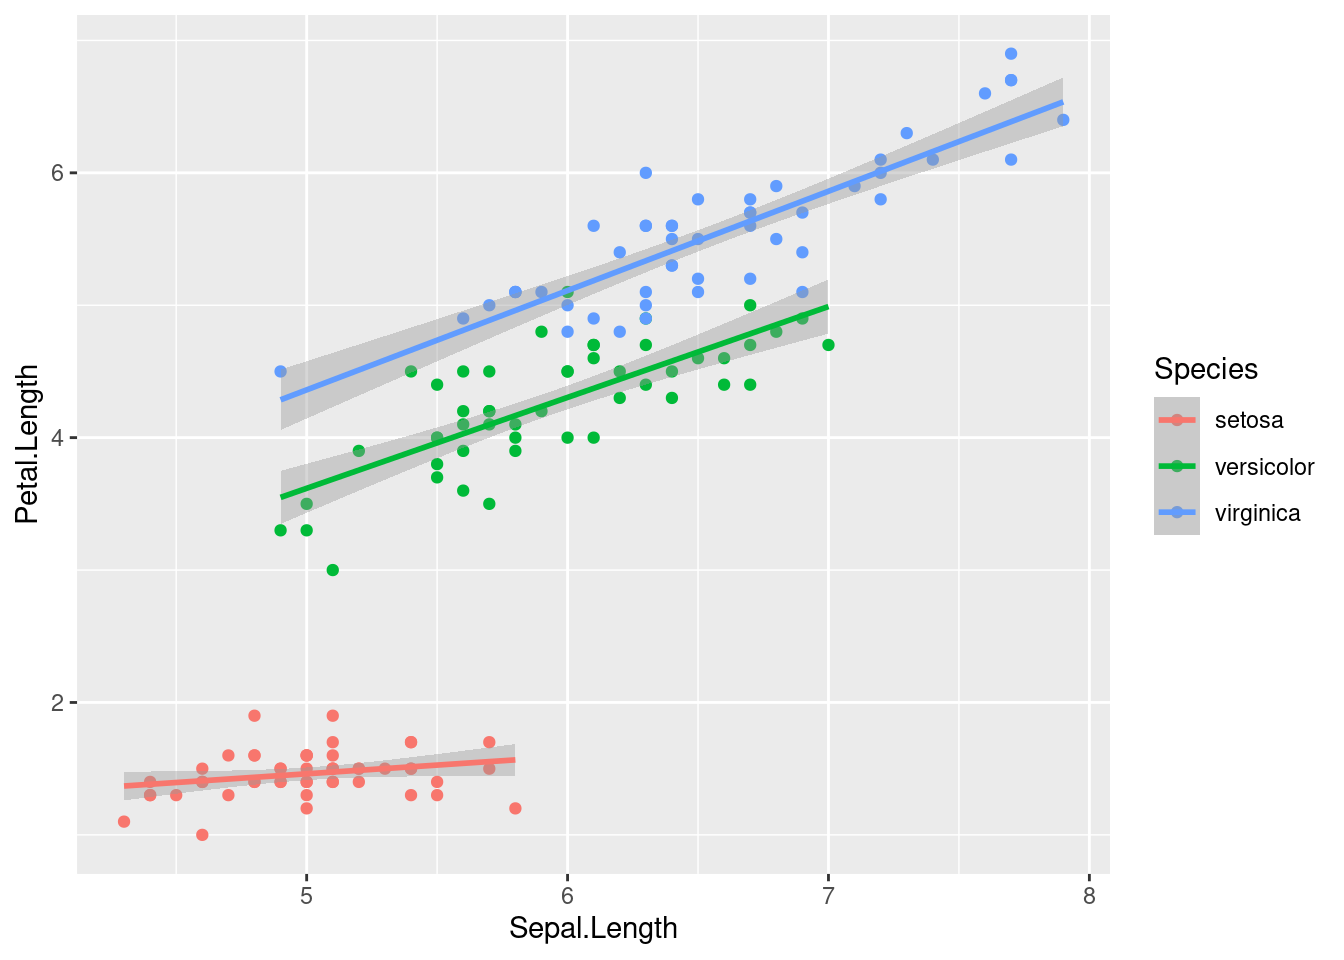
\includegraphics{Lecture1_files/figure-latex/unnamed-chunk-15-1}

Can we still estimate the hazard probability \(p\)?

\subsection{Probability distribution}\label{probability-distribution-1}

There are now 2 data streams. The first, \(X\), has the same
distribution as before: \[Pr(X = x) = f(x,p) = p(1-p)^{x-1}\]

The second \(Y\) will have value \(y\) as long as the actual event \(X\)
is greater than \(y\), so:

\[g(y,p) = Pr(Y = y) = Pr(X > y) = \sum_{i = y+1}^\infty p(1-p)^{i-1}\]

This is not as tidy as the non-censored example!

\subsection{Likelihood function}\label{likelihood-function-1}

The likelihood function now asks what is \(p\) given \(\bf X\), which
contains \(n\) known fate observations, and \(\bf Y\), which contains
\(m\) censored observations is:

\[{\cal L}(p|{\bf X},{\bf Y}) = \prod_{i=1}^n f(X_i|p) \prod_{i=1}^m g(Y_i|p)\]

The log likelihood is:

\[\begin{align} {\cal l}(p|{\bf X},{\bf Y})  &= \log({\cal L} (p|{\bf X},{\bf Y})) \\
 &= \sum_{i=1}^n \log(f(X_i|p)) + \sum_{i=1}^m \log(f(Y_i|p)) \end{align}\]

Ok, that's kind of a cop out. It's not so easy or necessary to write
out, but we can code it up using negative binomial short cuts. Namely
that \(f(x,p)\) is (very close to) the negative binomial
\emph{probability mass function}, and \(g(y,p)\) is one minus the
negative binomial \emph{cumulative mass function}.\footnote{THIS is
  where that differnece is important!}

\begin{Shaded}
\begin{Highlighting}[]
\NormalTok{p.censored.ll }\OtherTok{\textless{}{-}} \ControlFlowTok{function}\NormalTok{(p, Z, Y)\{}
    \CommentTok{\# true observations are the probability function dnbinom}
\NormalTok{    log.Z }\OtherTok{\textless{}{-}} \FunctionTok{dnbinom}\NormalTok{(Z}\DecValTok{{-}1}\NormalTok{, }\AttributeTok{prob =}\NormalTok{ p, }\AttributeTok{size =} \DecValTok{1}\NormalTok{, }\AttributeTok{log =} \ConstantTok{TRUE}\NormalTok{)   }
    \CommentTok{\# censored observations are the 1 {-} the cumulative probability pnbinom }
\NormalTok{    log.Y }\OtherTok{\textless{}{-}} \FunctionTok{log}\NormalTok{(}\DecValTok{1}\SpecialCharTok{{-}}\FunctionTok{pnbinom}\NormalTok{(Y}\DecValTok{{-}1}\NormalTok{, }\AttributeTok{prob =}\NormalTok{ p, }\AttributeTok{size =} \DecValTok{1}\NormalTok{))}
    \CommentTok{\# here, the log has to bo on the outside, can you see why?}
    \FunctionTok{sum}\NormalTok{(log.Z) }\SpecialCharTok{+} \FunctionTok{sum}\NormalTok{(log.Y)}
\NormalTok{\}}
\end{Highlighting}
\end{Shaded}

Note that in R, all distribution functions have a \texttt{log} option
\ldots{} now you maybe understand why:

Let's compare the likelihood function for both the full \(X\) dataset,
and the censored version:

\begin{Shaded}
\begin{Highlighting}[]
\NormalTok{ps }\OtherTok{\textless{}{-}} \FunctionTok{seq}\NormalTok{(}\FloatTok{1e{-}4}\NormalTok{,}\DecValTok{1}\FloatTok{{-}1e{-}4}\NormalTok{, }\AttributeTok{length =} \DecValTok{1000}\NormalTok{)}
\NormalTok{ll }\OtherTok{\textless{}{-}} \FunctionTok{sapply}\NormalTok{(ps, p.censored.ll, X, }\AttributeTok{Y =}\NormalTok{ Y)}
\NormalTok{ll.full }\OtherTok{\textless{}{-}} \FunctionTok{sapply}\NormalTok{(ps, p.ll, X.full)}
\FunctionTok{plot}\NormalTok{(ps, ll, }\AttributeTok{type =} \StringTok{"l"}\NormalTok{)}
\FunctionTok{lines}\NormalTok{(ps, ll.full, }\AttributeTok{col =} \DecValTok{2}\NormalTok{)}
\end{Highlighting}
\end{Shaded}

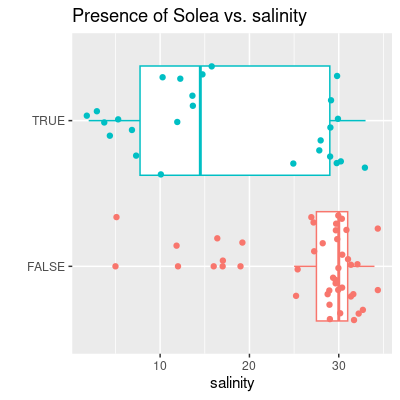
\includegraphics{Lecture1_files/figure-latex/unnamed-chunk-17-1}

\subsection{Maximum likelihood
estimate}\label{maximum-likelihood-estimate-1}

Using \texttt{optimize} to get the point estimate:

\begin{Shaded}
\begin{Highlighting}[]
\NormalTok{(p.hat }\OtherTok{\textless{}{-}} \FunctionTok{optimize}\NormalTok{(p.censored.ll, }\FunctionTok{c}\NormalTok{(}\DecValTok{0}\NormalTok{,}\DecValTok{1}\NormalTok{), }
                   \AttributeTok{Z =}\NormalTok{ X, }\AttributeTok{Y =}\NormalTok{ Y, }\AttributeTok{maximum =} \ConstantTok{TRUE}\NormalTok{))}
\end{Highlighting}
\end{Shaded}

\begin{verbatim}
## $maximum
## [1] 0.1115605
## 
## $objective
## [1] -84.64816
\end{verbatim}

\begin{Shaded}
\begin{Highlighting}[]
\NormalTok{p.dd }\OtherTok{\textless{}{-}} \FunctionTok{secondDeriv}\NormalTok{(p.hat}\SpecialCharTok{$}\NormalTok{maximum, p.censored.ll, }\AttributeTok{Z =}\NormalTok{ X, }\AttributeTok{Y =}\NormalTok{ Y)}
\NormalTok{se }\OtherTok{=} \FunctionTok{sqrt}\NormalTok{(}\SpecialCharTok{{-}}\DecValTok{1}\SpecialCharTok{/}\NormalTok{p.dd)}
\NormalTok{(}\AttributeTok{CI  =}\NormalTok{ p.hat}\SpecialCharTok{$}\NormalTok{maximum }\SpecialCharTok{+} \FunctionTok{c}\NormalTok{(}\SpecialCharTok{{-}}\DecValTok{2}\NormalTok{,}\DecValTok{2}\NormalTok{) }\SpecialCharTok{*}\NormalTok{ se[}\DecValTok{1}\NormalTok{,}\DecValTok{1}\NormalTok{])}
\end{Highlighting}
\end{Shaded}

\begin{verbatim}
## [1] 0.07108662 0.15203439
\end{verbatim}

Using \texttt{optim} instead:

\begin{Shaded}
\begin{Highlighting}[]
\NormalTok{p.fit }\OtherTok{\textless{}{-}} \FunctionTok{optim}\NormalTok{(}\FloatTok{0.5}\NormalTok{, p.censored.ll, }\AttributeTok{Z =}\NormalTok{ X, }\AttributeTok{Y =}\NormalTok{ Y, }
      \AttributeTok{control =} \FunctionTok{list}\NormalTok{(}\AttributeTok{fnscale =} \SpecialCharTok{{-}}\DecValTok{1}\NormalTok{), }
      \AttributeTok{hessian =} \ConstantTok{TRUE}\NormalTok{, }\AttributeTok{method =} \StringTok{"L{-}BFGS{-}B"}\NormalTok{, }
      \AttributeTok{lower =} \FloatTok{1e{-}7}\NormalTok{, }\AttributeTok{upper =} \DecValTok{1}\FloatTok{{-}1e{-}7}\NormalTok{)}

\NormalTok{p.hat }\OtherTok{\textless{}{-}}\NormalTok{ p.fit}\SpecialCharTok{$}\NormalTok{par}
\NormalTok{(p.se }\OtherTok{\textless{}{-}} \FunctionTok{sqrt}\NormalTok{(}\SpecialCharTok{{-}}\DecValTok{1}\SpecialCharTok{/}\NormalTok{p.fit}\SpecialCharTok{$}\NormalTok{hessian[}\DecValTok{1}\NormalTok{,}\DecValTok{1}\NormalTok{]))}
\end{Highlighting}
\end{Shaded}

\begin{verbatim}
## [1] 0.02023746
\end{verbatim}

\begin{Shaded}
\begin{Highlighting}[]
\FunctionTok{list}\NormalTok{(}\AttributeTok{p.hat =}\NormalTok{ p.hat, }\AttributeTok{p.CI =}\NormalTok{ p.hat }\SpecialCharTok{+} \FunctionTok{c}\NormalTok{(}\SpecialCharTok{{-}}\DecValTok{2}\NormalTok{,}\DecValTok{2}\NormalTok{) }\SpecialCharTok{*}\NormalTok{ p.se)}
\end{Highlighting}
\end{Shaded}

\begin{verbatim}
## $p.hat
## [1] 0.1115729
## 
## $p.CI
## [1] 0.07109795 0.15204777
\end{verbatim}

This is a horrible confidence interval! But it was also pretty brutal
censoring. Let's simulate a process and get a better feel for how things
can go:

\begin{Shaded}
\begin{Highlighting}[]
\FunctionTok{set.seed}\NormalTok{(}\DecValTok{1976}\NormalTok{)}
\NormalTok{X }\OtherTok{\textless{}{-}} \FunctionTok{rep}\NormalTok{(}\ConstantTok{NA}\NormalTok{, }\DecValTok{1000}\NormalTok{)}
\ControlFlowTok{for}\NormalTok{(i }\ControlFlowTok{in} \DecValTok{1}\SpecialCharTok{:}\FunctionTok{length}\NormalTok{(X))\{}
\NormalTok{    rolls }\OtherTok{\textless{}{-}} \DecValTok{0}
\NormalTok{    x }\OtherTok{\textless{}{-}} \DecValTok{0}
    \ControlFlowTok{while}\NormalTok{(x }\SpecialCharTok{!=} \DecValTok{6}\NormalTok{)\{}
\NormalTok{        rolls }\OtherTok{\textless{}{-}}\NormalTok{ rolls}\SpecialCharTok{+}\DecValTok{1}
\NormalTok{        x }\OtherTok{\textless{}{-}} \FunctionTok{sample}\NormalTok{(}\DecValTok{1}\SpecialCharTok{:}\DecValTok{6}\NormalTok{,}\DecValTok{1}\NormalTok{)}
\NormalTok{    \}}
\NormalTok{    X[i] }\OtherTok{\textless{}{-}}\NormalTok{ rolls}
\NormalTok{\}}
\NormalTok{X.full }\OtherTok{\textless{}{-}}\NormalTok{ X}
\NormalTok{Y }\OtherTok{\textless{}{-}} \FunctionTok{rep}\NormalTok{(}\DecValTok{6}\NormalTok{, }\FunctionTok{sum}\NormalTok{(X }\SpecialCharTok{\textgreater{}} \DecValTok{6}\NormalTok{))}
\NormalTok{X }\OtherTok{\textless{}{-}}\NormalTok{ X[X }\SpecialCharTok{\textless{}=} \DecValTok{6}\NormalTok{]}
\end{Highlighting}
\end{Shaded}

And estimate the full dataset:

\begin{Shaded}
\begin{Highlighting}[]
\NormalTok{p.fit }\OtherTok{\textless{}{-}} \FunctionTok{optim}\NormalTok{(}\FloatTok{0.5}\NormalTok{, p.ll, }\AttributeTok{X =}\NormalTok{ X.full, }
      \AttributeTok{control =} \FunctionTok{list}\NormalTok{(}\AttributeTok{fnscale =} \SpecialCharTok{{-}}\DecValTok{1}\NormalTok{), }
      \AttributeTok{hessian =} \ConstantTok{TRUE}\NormalTok{, }\AttributeTok{method =} \StringTok{"L{-}BFGS{-}B"}\NormalTok{, }
      \AttributeTok{lower =} \FloatTok{1e{-}7}\NormalTok{, }\AttributeTok{upper =} \DecValTok{1}\FloatTok{{-}1e{-}7}\NormalTok{)}
\NormalTok{p.hat }\OtherTok{\textless{}{-}}\NormalTok{ p.fit}\SpecialCharTok{$}\NormalTok{par}
\NormalTok{p.se }\OtherTok{\textless{}{-}} \FunctionTok{sqrt}\NormalTok{(}\SpecialCharTok{{-}}\DecValTok{1}\SpecialCharTok{/}\NormalTok{p.fit}\SpecialCharTok{$}\NormalTok{hessian[}\DecValTok{1}\NormalTok{,}\DecValTok{1}\NormalTok{])}
\FunctionTok{list}\NormalTok{(}\AttributeTok{p.hat =}\NormalTok{ p.hat, }\AttributeTok{p.CI =}\NormalTok{ p.hat }\SpecialCharTok{+} \FunctionTok{c}\NormalTok{(}\SpecialCharTok{{-}}\DecValTok{2}\NormalTok{,}\DecValTok{2}\NormalTok{) }\SpecialCharTok{*}\NormalTok{ p.se)}
\end{Highlighting}
\end{Shaded}

\begin{verbatim}
## $p.hat
## [1] 0.1596441
## 
## $p.CI
## [1] 0.1503886 0.1688996
\end{verbatim}

The censored dataset:

\begin{Shaded}
\begin{Highlighting}[]
\NormalTok{p.censored.ll }\OtherTok{\textless{}{-}} \ControlFlowTok{function}\NormalTok{(p, Z, Y)\{}
\NormalTok{    log.Z }\OtherTok{\textless{}{-}} \FunctionTok{dnbinom}\NormalTok{(Z}\DecValTok{{-}1}\NormalTok{, }\AttributeTok{prob =}\NormalTok{ p, }\AttributeTok{size =} \DecValTok{1}\NormalTok{, }\AttributeTok{log =} \ConstantTok{TRUE}\NormalTok{)   }
\NormalTok{    log.Y }\OtherTok{\textless{}{-}} \FunctionTok{log}\NormalTok{(}\DecValTok{1}\SpecialCharTok{{-}}\FunctionTok{pnbinom}\NormalTok{(Y}\DecValTok{{-}1}\NormalTok{, }\AttributeTok{prob =}\NormalTok{ p, }\AttributeTok{size =} \DecValTok{1}\NormalTok{))}
    \FunctionTok{sum}\NormalTok{(log.Z) }\SpecialCharTok{+} \FunctionTok{sum}\NormalTok{(log.Y)}
\NormalTok{\}}

\NormalTok{p.fit }\OtherTok{\textless{}{-}} \FunctionTok{optim}\NormalTok{(}\FloatTok{0.5}\NormalTok{, p.censored.ll, }\AttributeTok{Z =}\NormalTok{ X, }\AttributeTok{Y =}\NormalTok{ Y, }
      \AttributeTok{control =} \FunctionTok{list}\NormalTok{(}\AttributeTok{fnscale =} \SpecialCharTok{{-}}\DecValTok{1}\NormalTok{),}
      \AttributeTok{hessian =} \ConstantTok{TRUE}\NormalTok{, }\AttributeTok{method =} \StringTok{"L{-}BFGS{-}B"}\NormalTok{, }
      \AttributeTok{lower =} \FloatTok{1e{-}7}\NormalTok{, }\AttributeTok{upper =} \DecValTok{1}\FloatTok{{-}1e{-}7}\NormalTok{)}

\NormalTok{p.hat }\OtherTok{\textless{}{-}}\NormalTok{ p.fit}\SpecialCharTok{$}\NormalTok{par}
\NormalTok{p.se }\OtherTok{\textless{}{-}} \FunctionTok{sqrt}\NormalTok{(}\SpecialCharTok{{-}}\DecValTok{1}\SpecialCharTok{/}\NormalTok{p.fit}\SpecialCharTok{$}\NormalTok{hessian[}\DecValTok{1}\NormalTok{,}\DecValTok{1}\NormalTok{])}
\FunctionTok{list}\NormalTok{(}\AttributeTok{p.hat =}\NormalTok{ p.hat, }\AttributeTok{p.CI =}\NormalTok{ p.hat }\SpecialCharTok{+} \FunctionTok{c}\NormalTok{(}\SpecialCharTok{{-}}\DecValTok{2}\NormalTok{,}\DecValTok{2}\NormalTok{) }\SpecialCharTok{*}\NormalTok{ p.se)}
\end{Highlighting}
\end{Shaded}

\begin{verbatim}
## $p.hat
## [1] 0.1624736
## 
## $p.CI
## [1] 0.1508277 0.1741195
\end{verbatim}

Only the observed dataset:

\begin{Shaded}
\begin{Highlighting}[]
\NormalTok{p.fit }\OtherTok{\textless{}{-}} \FunctionTok{optim}\NormalTok{(}\FloatTok{0.5}\NormalTok{, p.ll, }\AttributeTok{X =}\NormalTok{ X, }
      \AttributeTok{control =} \FunctionTok{list}\NormalTok{(}\AttributeTok{fnscale =} \SpecialCharTok{{-}}\DecValTok{1}\NormalTok{),}
      \AttributeTok{hessian =} \ConstantTok{TRUE}\NormalTok{, }\AttributeTok{method =} \StringTok{"L{-}BFGS{-}B"}\NormalTok{, }
      \AttributeTok{lower =} \FloatTok{1e{-}7}\NormalTok{, }\AttributeTok{upper =} \DecValTok{1}\FloatTok{{-}1e{-}7}\NormalTok{)}

\NormalTok{p.hat }\OtherTok{\textless{}{-}}\NormalTok{ p.fit}\SpecialCharTok{$}\NormalTok{par}
\NormalTok{p.se }\OtherTok{\textless{}{-}} \FunctionTok{sqrt}\NormalTok{(}\SpecialCharTok{{-}}\DecValTok{1}\SpecialCharTok{/}\NormalTok{p.fit}\SpecialCharTok{$}\NormalTok{hessian[}\DecValTok{1}\NormalTok{,}\DecValTok{1}\NormalTok{])}
\FunctionTok{list}\NormalTok{(}\AttributeTok{p.hat =}\NormalTok{ p.hat, }\AttributeTok{p.CI =}\NormalTok{ p.hat }\SpecialCharTok{+} \FunctionTok{c}\NormalTok{(}\SpecialCharTok{{-}}\DecValTok{2}\NormalTok{,}\DecValTok{2}\NormalTok{) }\SpecialCharTok{*}\NormalTok{ p.se)}
\end{Highlighting}
\end{Shaded}

\begin{verbatim}
## $p.hat
## [1] 0.3387017
## 
## $p.CI
## [1] 0.3171283 0.3602751
\end{verbatim}

This is a huge overestimate, and shows the importance of taking the
censored data into account!

\section{Next time \ldots{}}\label{next-time}

we discuss how to generalize these principles to \textbf{continuous time
to event} modeling, which is much more common / practical.



\end{document}
